\section{Trac}
\fib{}

\noindent
Trac ist eine Software die bei der Entwicklung und Organisation des Projekts eine große Hilfe ist. Dadurch wird ein Interface für Versionsverwaltung geboten, sowie ein für Scrum ideales Ticketsystem. Außerdem bietet es einen Aktivitätsüberblick und einen Überblick über den aktuellen Stand des Projekts in Form von einer Roadmap.
\footcite{noauthor_trac_nodate}

\noindent
Durch das Ticketsystem kann man mit Leichtigkeit die verschiedenen Aufgaben verteilen und feststellen ob sie fertiggestellt wurden.
\\
\begin{figure}[h]
	\begin{center}
		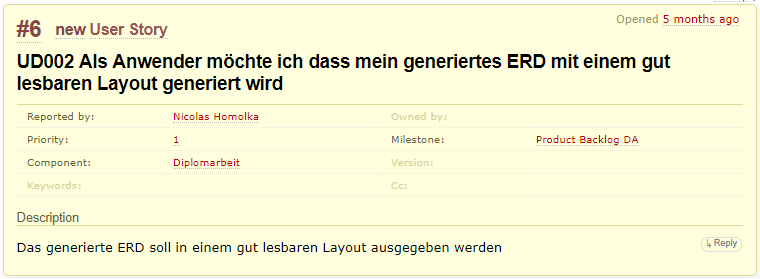
\includegraphics[width=16cm]{images/Trac_Tickets.png}
		\caption{Ticket im Trac}
		\label{Trac Ticket}
	\end{center}
\end{figure}

\noindent
Trac unterstützt WikiFormatting, mithilfe diesem Merkmals kann man eine angenehme und leicht leserliche Struktur erschaffen.

\noindent
Davon war das erstellen von Links auf interne Ressourcen sowie auf externe Ressourcen eine der meist verwendeten Funktionen.
\begin{figure}[h]
	\begin{center}
		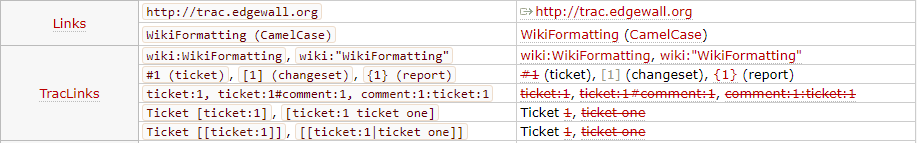
\includegraphics[width=16cm]{images/Trac_Links.png}
		\caption{Dokumentation für Links im Trac}
		\label{Trac Links}
	\end{center}
\end{figure}